\chapter{Graph Attention Networks Embedded Knowledge Tracing Model With Transformer}

% **************************** Define Graphics Path **************************
\ifpdf
	\graphicspath{{Chapter3/Figs/Raster/}{Chapter3/Figs/PDF/}{Chapter3/Figs/}}
\else
	\graphicspath{{Chapter3/Figs/Raster/}{Chapter3/Figs/Vector/}{Chapter3/Figs/PDF/}{Chapter3/Figs/}}
\fi

\section{Research Motivation}
%本章节为该推荐系统的一个核心部分,即通过知识追踪的方式获取学生的知识掌握状态。知识追踪是根据学生的以往的答题记录来建模学生的知识掌握情况,从而获取学生的知识状态。知识追踪的模型非常丰富,早期的知识追踪模型贝叶斯知识追踪(BKT),它们的基础假设是学生答题基于一系列知识点,这些知识点之间被认为是相互不相关的,因此它们之间是独立表示,这种做法无法捕捉不同概念之间的关系也无法表征复杂的概念转换。在2015年,Piech等人提出了深度知识追踪模型(DKT),首次将长短期记忆网络(LSTM)应用于知识追踪任务,它无需进行知识点标注,而是包含一个知识的隐含状态,当时取得了超过BKT的基线性能,它标志着基于神经网络模型的知识追踪研究的序幕。但DKT无法输出知识的隐藏状态,可解释性不足。而且DKT用将所有记忆存储于一个隐藏向量中,对于长序列的预测性能不够理想。针对这个问题,记忆增强网络(MANN)被提出来,它允许网络保留多个隐藏状态向量,并分别读写这些向量。在2017年,张等人提出了Dynamic Key-Value Memory Networks(DKVMN),它参考了MANN的设计,针对知识追踪任务进行了优化,优化了MANN对于知识追踪任务的输入输出不同域的问题。DKVMN采用了键值对作为存储器结构,能避免过拟合、参数少,以及通过潜在概念自动发现相似练习,取得了相对BKT和DKT更好的预测性能。同时该模型也具有较好的可解释性,它将问题相关潜在概念存储于键矩阵中,对概念掌握程度存储于值矩阵中,通过对输入练习与键矩阵的相关性对值矩阵进行更新。但这些模型仍存在长依赖的问题。为了解决这个问题,设计了一个hop-LSTM结构来聚合相似的习题的隐藏状态的Sequential Key-Value Memory Networks(SKVMN)被提出来。但现有的模型往往对于知识点之间的高阶连接考虑不足,或者简单地将知识点作为相互独立的节点,或者将知识点作为简单的层次模型,但实际上,知识点之间是高阶的图状结构,在这种情况下,采用图神经网络来表征知识点之间的关系,训练问题embedding和概念embedding是更好的选择,因此在本章,我们提出了基于图神经网络的知识追踪模型,它利用高阶问题-知识点关系,来解决稀疏性和复杂知识点依赖问题,同时,它通过问题日志模块,可以学习学生的掌握速度,从而更好表征知识追踪过程。

This section is a core part of this recommendation system to obtain the student's knowledge mastery status using knowledge tracing. Knowledge tracing is used to model students' knowledge mastery based on their previous answer records to obtain their knowledge status. There is a wealth of models for knowledge tracing, early models of knowledge tracing Bayesian Knowledge Tracing (BKT)~\cite{yudelson2013individualized}, which issued the assumption that students' solutions to exercises are based on a set of knowledge points that are considered to be unrelated to each other and are therefore represented independently of each other. This approach fails to capture the relationships between different concepts nor to characterize complex conceptual transformations. In 2015, Piech et al. proposed the deep knowledge tracing model (DKT), which first applied RNN to the knowledge tracing task, which contains an implicit state of knowledge, and achieved a baseline performance over BKT at that time, and it marked the prologue of knowledge tracing research based on neural network models. However, DKT cannot output the hidden state of knowledge and is not sufficiently interpretable.
Moreover, DKT uses to store all memories in a hidden vector, and the prediction performance for long sequences is not satisfactory enough. Memory Augmented Neural Network (MANN)~\cite{santoro2016meta} was proposed to address this problem, which allows the network to keep multiple hidden state vectors and read and write these vectors separately. In 2017, Dynamic Key-Value Memory Networks (DKVMN)~\cite{zhang2017dynamic} referring to the design of MANN for knowledge tracing tasks and optimizes MANN for knowledge tracing tasks with different input and output domains. DKVMN uses key-value pairs as the memory structure, which can avoid over better prediction performance relative to BKT, and DKT is achieved by using key-value pairs as the memory structure, which can avoid overfitting. The model also has better interpretability. It stores the problem-related potential concepts in the key matrix and the mastery proficiency to the concepts in the value matrix and updates the value matrix by correlating the input exercises with the key matrix. However, these models still suffer from the problem of long dependencies. Sequential Key-Value Memory Networks (SKVMN)~\cite{Abdelrahman_2019}, which designs a hop-LSTM structure to aggregate the hidden states of similar exercises, was proposed. However, existing models often do not consider enough the higher-order connections between knowledge points, or treat knowledge points as mutually independent nodes, or treat knowledge points as simple hierarchical models. However, knowledge points are higher-order graph-like structures, in which case, using graph neural networks to characterize the relationships between knowledge points, training problem embedding and concept embedding is a better choice, so in this chapter, a graph neural network-based knowledge tracing model, which uses higher-order problem-knowledge point relationships to solve the sparsity and complex knowledge point dependency problems, and at the same time, it can learn the mastery speed of students through the problem logging module, to better characterize the knowledge tracing process.

\section{Related Theory}
\subsection{Knowledge Tracing}
%知识追踪为智能化和自适应教育提供了条件,它具有个性化和自动化的特点。知识追踪任务从学生的历史学习记录来追踪学生的知识状态变化,预测未来的学习表现,从而针对性地给予学习辅导。其本质基于学生的过去的学习表现来获取当前的学习状态,从而预测将来的学习表现。其实际做法是,对学生过去的答题记录进行数据分析和过程建模,从而建模当前的学生学习状态数据,让模型跟做学生的每个阶段的学习状态,并基于学习状态数据来预测习题答对的概率。在学科学习中,学科知识由一系列知识点组成,学生的学习状态实际上基于对于各个知识点的掌握情况。而知识追踪一般的形式为给定一个学生的答题序列,该序列由一系列习题构成,习题又与特定的知识点相关联,在知识追踪中的一个基本假设是,学生的答题表现基于对知识点的掌握。而学生的答题表现即可用于反推学生对于各个知识点的掌握情况,即学习状态的掌握情况。

%知识追踪任务的数学表示为一个学生在一个习题序列上的交互式答题记录\(X_t=(x_1,x_2,\ldots,x_t)\),根据该记录通过建模来获取学生的学习状态,并预测学生在下一次练习中的表现$x_{t+1}$。其中$x_t$通常表示为一个有序对$(q_t,a_t)$,有序对表示学生在时间$t$回答了问题$q_t$,$a_t$表示问题的得分情况,也有许多知识追踪任务用答对或答错来表示,此时$a_t$为0或者1,在此情况下,实际上预测的是对于下一个问题回答正确的概率$P(a_{t+1}=1|a_t)$。如图ref{kt1}。


Knowledge tracing provides the conditions for intelligent and adaptive education, which is personalized and automated. Knowledge tracing tracks students' knowledge status from their historical learning records, predicts future learning performance and provides targeted learning coaching. The essence is to obtain the current learning status based on the student's past learning performance to predict the future learning performance. The actual practice is to analyze the data and process modeling of students' past answer records to model the current student learning status data and let the model follow the learning status of students at each stage, and predict the probability of correct answers to the exercises based on the learning status data. In subject learning, subject knowledge consists of a series of knowledge points, and students' learning status is based on their mastery proficiency to each elementary knowledge concept. The general form of knowledge tracing is that given a sequence of student answers, which consists of a series of exercises associated with a specific knowledge point, a fundamental assumption in knowledge tracing is that student performance is based on mastery proficiency to the knowledge concept. The student's performance can be applied to infer the student's mastery proficiency for each knowledge concept, i.e., the mastery proficiency to the learning state.

The mathematical representation of the knowledge tracing task is an interactive answer record \(X_t=(x_1,x_2,\ldots,x_{t-1})\) of a student on an exercise sequence, based on which the student's learning status is obtained by modeling and predicting the student's performance in the next exercise \(x_{t}\). Where \(x_t\) is usually represented as an ordered pair \((q_t,a_t)\), the ordered pair indicates that the student answered the exercise \(q_t\) at time \(t\), and \(a_t\) indicates the score of the exercise, also many knowledge tracing tasks are represented by correct or incorrect answers, when \(a_t\) is 0 or 1. In this case, what is actually predicted is the probability of answering correctly for the next exercise \(P(a_{t}=1|a_{t-1},\ldots,a_1)\). As shown in the figure \figurename{\ref{fig:ch3-model-ktdes}}.

\begin{figure}
	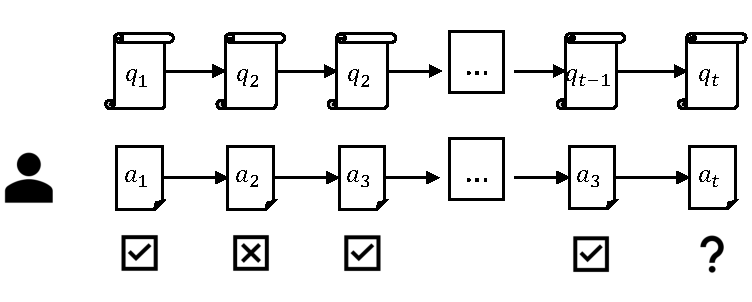
\includegraphics[width=0.9\textwidth]{ch3-model-ktdes.pdf}
	\caption{The knowledge tracing pattern}\label{fig:ch3-model-ktdes}
\end{figure}

\subsection{Graph Neural Networks}
%在提取欧氏空间数据特征方面取得了较大成功的传统神经网络模型,在非欧氏空间上的应用却效果并不理想。而目前,许多实际的应用场景正式非欧式空间生成的。在知识追踪过程中,知识点之间的联系正是一种非欧式空间的结构,即知识图结构。图的不规则性和复杂性对于传统的深度学习算法提出了巨大的挑战,图的节点的联系的可变性导致了庞大的计算量,这使得一些在欧氏空间表现良好的传统神经网络模型无法直接应用于非欧式空间。例如,在处理图像中,图像的每个像素都是相互独立的,卷积神经网络对于图像这种稳定单一且个部分相互独立的结构较为容易计算和并行化,但对于每个节点都与其他节点联系并有依赖关系的图结构来说,情况并非如此。为了表征图节点之间相互依赖的关系,图神经网络(GNN)被提出来。 GCN作为图神经网络的开山之作,将图像处理中的卷积操作简单的用到图结构数据处理中来,并且给出了具体的推导。它实际上是聚合图邻居节点的特征做一个线性变换。为了能够解决图传播深度不足的问题,还可以堆叠多层GCN层以捕捉k-hop的邻居节点信息。GCN通过对于图的结构的编码取得了优秀的节点表征性能。但GCN的处理方式需要将整个图放到计算显存内,这限制了其计算性能。且它需要预先输入图的结构信息,这限制了它的应用。为了解决GCN聚合邻居节点忽略不同邻居节点的权重不同的问题, Graph Attention Networks(GAT) 引入了masked self-attention机制,计算每个节点的表示时,根据邻居节点特征来分配不同权值。它无需使用预先构建好的图,因此只需要知道邻居节点即可,这大大增加了计算速度。

%图嵌入是一个图神经网络的重要研究课题,它通过保留图的网络拓扑结构和节点信息,将图中节点表示为低维向量,然后通过其他的机器学习算法进行处理。在本章中,我们通过一个图嵌入算法来表征知识点之间的关联和知识点信息,从而获取对于知识结构的嵌入学习。

The traditional neural network model, which has achieved tremendous success in extracting Euclidean space data features, has not worked well for non-Euclidean space applications. Moreover, currently, many practical application scenarios are formally generated in non-Euclidean spaces. In the process of knowledge tracing, the connection between knowledge points is exactly a structure of non-Euclidean space, i.e., knowledge graph structure. The irregularity and complexity of graphs pose a significant challenge to traditional deep learning algorithms, and the variability of the connections of the nodes of graphs leads to a massive computational effort, which makes some traditional neural network models that perform well in Euclidean space cannot be directly applied to non-Euclidean space. e.g., in processing images where each pixel of the image is independent of each other, convolutional neural networks are easier to compute and parallelize for structures like images that are stable and single and have individual parts independent of each other, but this is not the case for graph structures where each vertex is connected to and has dependencies on other nodes. Graph-based Networks are proposed to characterize the interdependencies between graph nodes.

As the pioneer of graph neural networks, GCN applies the convolution operation in image processing to graph-structured data processing and gives a specific derivation. It aggregates the features of graph neighbor nodes to make a linear transformation. Multiple GCN layers can be stacked to capture the k-hop neighbor vertex information to solve the problem of insufficient depth of graph propagation. However, GCN processing requires putting the whole graph into the computational memory, limiting its computational performance. It also requires pre-inputting the graph structure information, which limits its application. To solve the problem, GCN aggregates neighbor nodes ignoring different neighbor nodes' weights, Graph Attention Networks (GAT) attention algorithm to compute each vertex's representation. It does not need to use a pre-constructed graph, so only the neighbor nodes need to be known, significantly increasing the computational speed.

Graph embedding is an important research topic in graph neural networks, representing nodes in a graph as low-dimensional vectors by preserving the network topology and vertex information of the graph, which is then processed by other machine learning algorithms. In this chapter, the association between knowledge points and knowledge point information by a graph embedding algorithm to obtain the learning of embedding for knowledge structures is characterized.

% \subsection{Transformer}


\section{Proposed Model}
\subsection{Algorithm Overview}
%本节的关键点是对学生的知识追踪,本文提出了一种基于图自注意力网络和Transformer模型的知识追踪模型GATKT。在实验验证阶段,该模型在几个数据集上的基线性能达到了SOA。本模型的第一层为embedding聚合层,该层用一个GAT来聚合问题embedding和知识点embedding,并展示问题和知识点的内在联系,它可以解决数据稀疏性问题和知识点依赖和复杂关系问题。第二层为一个Transformer-based知识追踪模型,该层参考Google提出的著名的Transformer模型 ~\cite{vaswani2017attention},设计了一个基于Transformer机制的知识追踪模型,它输入问题和技能embedding,输出对于下一个问题的答对的预测。通过这种机制,该模型可以实现对long-range的依赖的学习。此外,本模型可以通过解码器来输出隐藏的知识状态,这是下一阶段进行习题推荐的关键。总而言之,该模型的总体架构图可以见图\ref{},并分为以下几个模块。
%1. 基于GAT的embedding层:该层用embedding方法来表征问题,知识点和回答。在该图神经网络中,每个问题代表一个节点,它与若干知识点节点连接,这些知识点节点再与与之相关的问题节点连接。而问题与问题不直接连接,考虑到知识点的相关性,知识点与知识点可以直接连接。其结构如图\ref{}。这个embedding层不进行预训练,而是与其他层进行总体训练来优化最终结果。
%2. 基于Transformer的知识状态表征:该模块通过多头注意力机制来学习经过GAT嵌入表示的习题-知识点向量,并学习学生做题记录过程中的知识状态表征。
%3. 基于Transformer的知识追踪层:该层类似传统Transformer结构,具有encoder和decoder两部分,它学习关联知识点和问题的权值矩阵,可以解决知识点依赖问题。通过注意力机制,它也可以capture关联知识点相似的问题。

The key point of this section is to track students' knowledge. What is issued is a knowledge tracing model based on graph attention network and Transformer model. In the experimental verification phase, the baseline performance of the model on several datasets achieves SOTA performance. The first layer of this model is the embedding aggregation layer. In this layer, a GAT embedding is used to aggregate the problem embedding and the knowledge point embedding and how the internal relationship between the problem and the knowledge point. It can solve the problem of knowledge point dependence and complex relationships. The second layer is a transformer-based knowledge tracing model. Referring to the famous transformer model proposed by Google Brain~\cite{vaswani2017attention}, this layer designs a knowledge tracing model with Transformer-structure, which inputs exercises and skills embedding and outputs the prediction correctness to the next exercise. Through this mechanism, the model can realize the learning of long-range dependence. Also, the model can output the hidden knowledge state through the Decoder, which is the Key to exercise recommendation in the next stage. In a word, the overall architecture diagram of the model is in \figurename{\ref{fig:ch3-fig1}}, which is segmented into the following modules:
\begin{enumerate}
	\item GAT-based embedding layer: embedding layer based on gat: this layer uses the embedding method to represent exercises, knowledge points, and answers. In the graph neural network, each problem represents a vertex connected with several knowledge nodes, and these knowledge nodes are connected with the related problem nodes. Due to the relevance of knowledge points, they can be directly connected with other ones. The structure is shown in the \figurename{\ref{fig:ch3-fig2}}. This embedding layer does not carry out pre-training but carries out overall training with other layers to optimize the final result.
	\item Transformer-based knowledge state encoder: this layer establishes a graph of knowledge points applied to track the students' mastery proficiency to knowledge points. This layer updates the knowledge state through the knowledge state, and finally, it will be applied in the subsequent recommendation process.
	\item Knowledge tracing layer based on Transformer: this layer is similar to the traditional transformer structure and has two parts: encoder and Decoder. It learns the weight matrix of knowledge points and problems and can solve knowledge point dependence. Through the attention mechanism, it can also capture similar problems of knowledge points.
\end{enumerate}

\begin{figure}[htbp!]
	\centering
	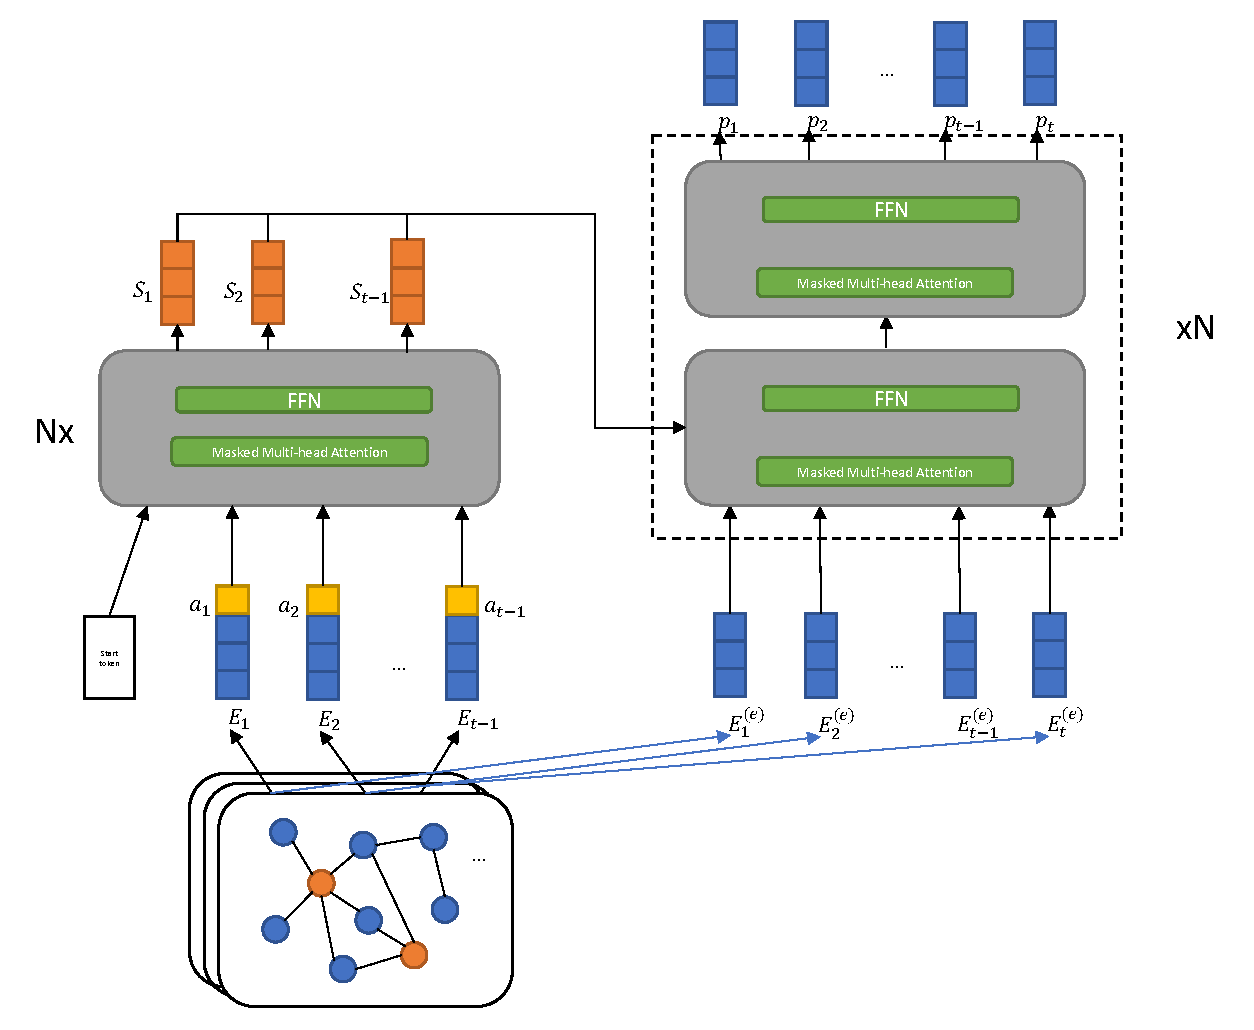
\includegraphics[width=0.9\textwidth]{ch3-overview.pdf}
	\caption{Overview Model Structure}\label{fig:ch3-fig1}
\end{figure}
\begin{figure}[htbp!]
	\centering
	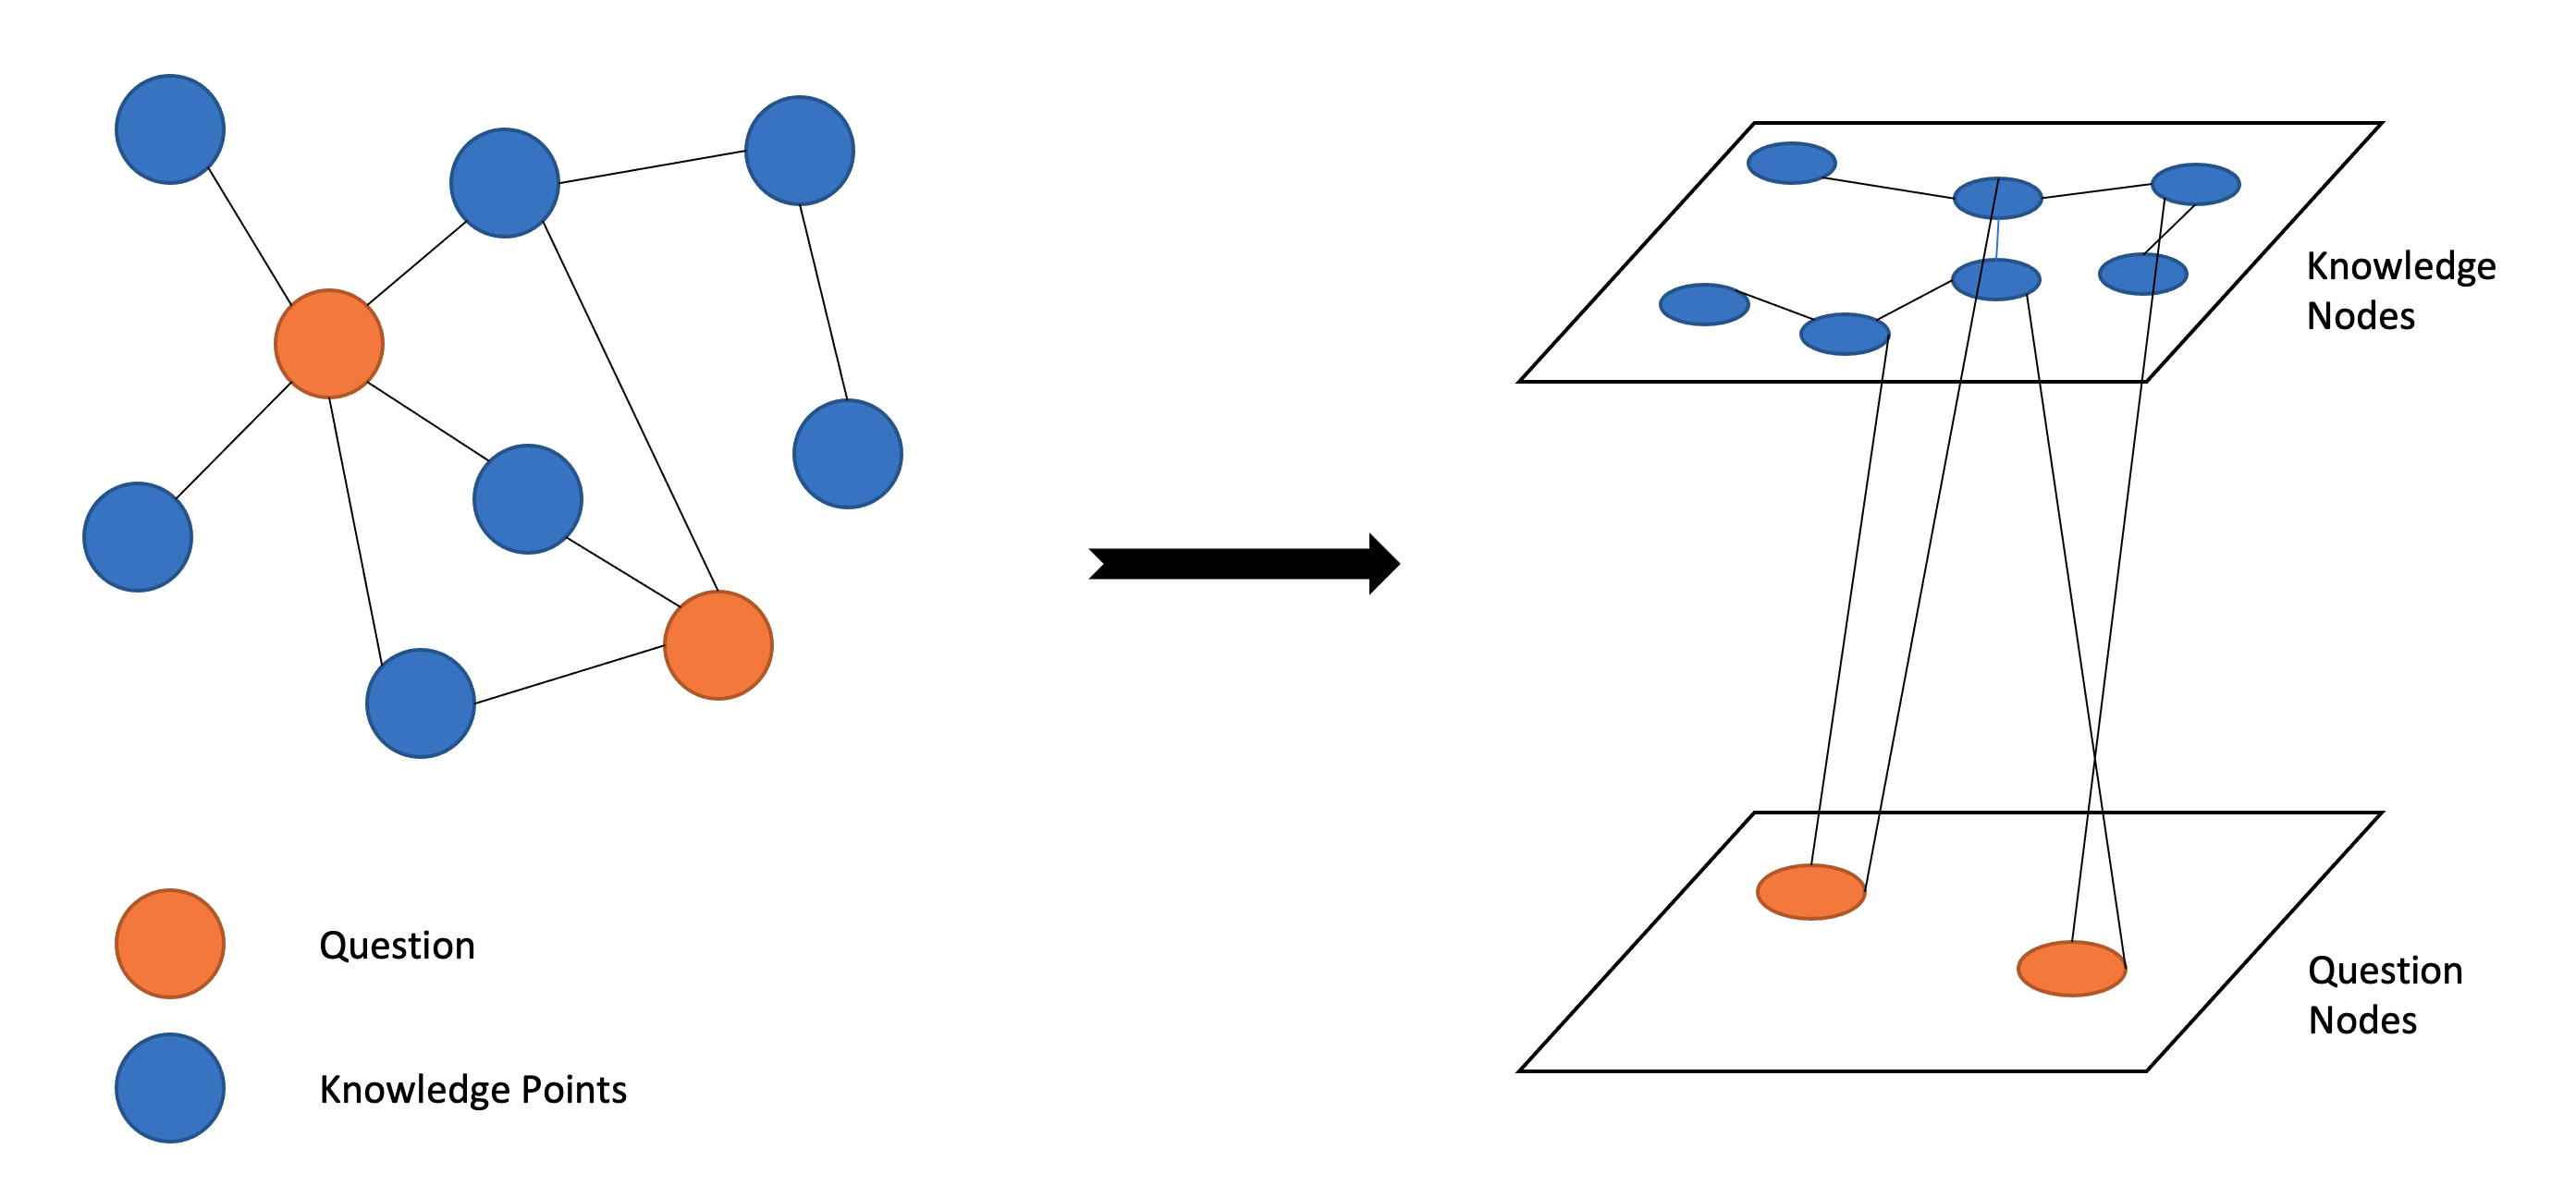
\includegraphics[width=0.9\textwidth]{ch3-fig2.png}
	\caption{The Graph of Knowledge Point and exercise}\label{fig:ch3-fig2}
\end{figure}


\subsection{GAT-based Embedding Layer}
%本节中,采用了图自注意力网络来对问题-知识点关联图进行embedding。它用于降低表征问题数据中知识点的数据稀疏性。我们把第i个问题记作$q_i$,学生对第i个问题的回答记作$a_i$,回答的结果为对或者错,则可以将其记作$a_i\in\{0,1\}$,则答题记录记为$X=\{x_1,x_2,...x_{t-1}\}$,其中$x_i=(q_i,a_i)$,我们基于前$t-1$次的答题记录来预测第$t$题的回答正确概率。对于每个问题$q_i$,有一系列的知识点与之相关,这些知识点记作$\{p_1,p_2,...,p_{n_i}\}$。在这里进行embedding计算可以获取问题之间的深层次关联关系,即知识点的相关性。用图结构可以较为理想地做到这一点。从直观上来说,也可以通过对于知识点的掌握情况来推知问题的答对概率。该方法也可以建立对于问题-知识点的更好的表征。

In this section, a graph self-attention network (GAT) is introduced to embed the problem-knowledge point association graph, which can reduce the data sparsity of the knowledge points in the problem data. The ith exercise can be recorded as \(q_i\), the student's answer to the ith exercise as \(a_i\), and the answer is correct or wrong, so it can be recorded as \(a_i\in \{0,1\} \), the answer record is recorded as \(X=\{x_1,x_2,\ldots,x_{t-1}\} \), where \(x_i=(q_i,a_i)\). It is based on the previous \(t-1\) times to predict the exercise's correctness in \(t\). For each exercise \(q_i\), there are a series of knowledge points related to it. These knowledge points are denoted as \( \{p_1,p_2,\ldots,p_{n_i}\} \). The embedding calculation can obtain the deep-level relationship between the problems, i.e., the relevance of knowledge points. This can be done ideally with a graph structure. Intuitively, you can also infer the probability of answering the exercise through mastery proficiency to the knowledge points. This method can also establish a better representation of the problem-knowledge point.

Embedding calculation can obtain the deep correlation between problems, i.e., the correlation of referred knowledge points. This can be achieved with graph structure. Intuitively speaking, it also infers the correct answer probability of the exercise by mastering the knowledge points. This method can also establish a better representation of problem knowledge points. In the exercise-knowledge graph, GAT can capture the high order relation for n-hop neighboring nodes. Also, GAT uses the idea of Transformer for reference and introduces a masked self-attention mechanism. When calculating each vertex's representation in the graph, it will assign different weights to its neighbors according to their different characteristics.

GAT applies an attention mechanism to the weighted summation of neighboring vertex features. The weights of the neighboring vertex features depend entirely on the vertex features and are independent of the graph structure. In GAT, each vertex in the graph can be assigned different weights to neighboring nodes based on their characteristics. With the introduction of the attention mechanism, it is only relevant to adjacent nodes, i.e., nodes that share edges, without getting information about the whole graph. Specifically, the vertex of the GAT network represents the knowledge point embedding or exercise embedding.

%提出的方法将习题都作为GAT的节点。对于习题\(i\),输入特征为\(\overrightarrow{h^(e)}_i\),特征包括习题位置,习题的作答正确性,以及习题包含的知识点。可以从习题类别来建立习题的邻接矩阵\(A\),即当多个习题为同一类,则为邻居节点,这样进行预处理可以减少后续的计算量,防止无效的连接带来的干扰。例如当习题1与习题3都属于线性代数这个类别,则\(A[1,3]=1\),它们会在图计算中进行特征聚合。GAT的输入层可以写作\(\mathbb{h^{(e)}}_0=\{\overrightarrow{h^{(e)}}_1,\overrightarrow{h^{(e)}}_2,\ldots,\overrightarrow{h^{(e)}}_{\mathcal{V}^i}\} \)

The proposed method treats all the exercises as nodes of GAT. For the exercises \(i\) in an exercise set of size \(N^{(e)}\), the input features are \(\overrightarrow{h}^{(e)}_i\), and the features include the location of the exercises, the correctness of the answers to the exercises, and the knowledge points contained in the exercises. The adjacency matrix \(A\) of the exercises can be established from the exercises category, i.e., when multiple exercises are of the same category, they are neighbor nodes, so preprocessing can reduce the subsequent computation and prevent the interference caused by invalid connections. For example, when both Exercise 1 and Exercise 3 belong to the category of linear algebra, \(A[1,3]=1\), they will be aggregated in the graph computation for features. The neighboring vertex set of vertex \(i\) is marked as \(\mathcal{V}^i\). Input of GAT can be denoted as \(\mathbf{h}^{(e)}_0=\{\overrightarrow{h}^{(e)}_{0,1},\overrightarrow{h}^{(e)}_{0,2}\ldots,\overrightarrow{h}^{(e)}_{0,N^{(e)}}\} \), in which \(\overrightarrow{h}^{(e)}_i\in\mathbb{R}^{F^{(e)}}\) and \(F^{(e)}\) is the amount of feature of exercise.

To achieve better high dimension feature representation, at least one linear transformation from low-dimensional should be embedded to high-dimensional features. Therefore, a linear transformation is first done for the vertex features and then the coefficients are calculated. The attention mechanism of self-attention is implemented for each vertex, and the attention coefficients (Attention coefficients) and its softmax value are calculated in formula~\ref{fml:gatembeij} and~\ref{fml:gatembalphaij}:


\begin{align}
	e_{ij}      & =a(\mathbf{W}_l\overrightarrow{h}^{(e)}_i, \mathbf{W}_l\overrightarrow{h}^{(e)}_j)    \label{fml:gatembeij}                \\
	\alpha_{ij} & =\operatorname{softmax}_{j}(e_{ij})=\frac{\exp(e_{ij})}{\sum_{k\in \mathcal{N}_{i}}\exp(e_{ik})} \label{fml:gatembalphaij}
\end{align}
The \(e_{ij}\) is the contribution degree from vertex \(i\) to vertex \(j\) and the \(\alpha_{ij} \) is the normalized contribution degree, and the \(\mathbf{W}_l\) is the ith layer's weight matrix. Here, since the graph structure information is to be considered, the concept of masked attention is introduced, which means that the denominator of the softmax considers only the first-order information about the neighbors. By this method, each vertex then gets a weight about the neighboring nodes, and then the combined representation of the nodes is obtained by summing. That is, the attention weighted summing can be calculated to generate aggregate neighboring features. The relative formula is~\ref{fml:gatwsum}, where \(\sigma \) are the non-linear transformation such as ReLU or LeakyReLU. If the edge \(j \to i\) does not exist,  the calculation of \(\alpha_{ij}\), which can reduce the calculation, can be performed. The formula means that this vertex's output characteristics are related to all the nodes adjacent to it and are obtained after the nonlinear activation of their linear sum.

\begin{align}
	\overrightarrow{h}^{(e)}_{l+1,i}=\sigma(\sum_{j \in \mathcal{N}^i} \alpha_{i j} \mathbf{W}_l \overrightarrow{h}^{(e)}_{i,j})\label{fml:gatwsum}
\end{align}

% The procedure is like \figurename{\ref{fig:ch3-gat-emb}};

% \begin{figure}[htbp!]
% 	\centering
% 	\includegraphics[width=0.9\textwidth]{ch3-emb.png}
% 	\caption{Feature extraction and attention mechanism}\label{fig:ch3-gat-emb}
% \end{figure}

To make the result of self-attention more stable. The multi-headed attention mechanism can be used here.\(K\) independent attention mechanisms can be achieved by connecting \(k\) features together. The formula is like~\ref{fml:gat-emb2}.

\begin{align}
	\overrightarrow{h}^{(e)}_{l+1,i}=\|_{k=1}^{K} \sigma(\sum_{j \in \mathcal{N}^i} \alpha_{i j}^{k} \mathbf{W}_l^{k} \overrightarrow{h}^{(e)}_{i,j})\label{fml:gat-emb2}
\end{align}

K-averaging is used to replace the join operation and to delay the application of the final nonlinear function. The attention coefficients between different nodes after regularization are obtained by the above operation and can predict each vertex's characteristics. The formula is like~\ref{fml:gat-emb2}.

\begin{align}
	\overrightarrow{h}^{(e)}_{l+1,i}=\sigma(\frac{1}{K} \sum_{k=1}^{K} \sum_{j \in \mathcal{N}^i} \alpha_{i j}^{k} \mathbf{W}_l^{k} \overrightarrow{h}^{(e)}_{i,j})\label{fml:gat-emb3}
\end{align}

From L-layer GAT, the embedded vector of exercise \(i\) are denoted as \(E^{(e)}_i = \overrightarrow{h}^{(e)}_{L, i}\), which would be passed into the Transformer Block in Knowledge tracing module.

\subsection{Transformer Based Knowledge Tracing}
The input of transformer Block is the concatenation of the embedded exercise \(E^{(e)}_i \) and corresponding answer correctness \(a_i\), i.e. \(E_i=E^{(e)}_i\|a_i\). The general structure is like \figurename{\ref{fig:ch3-fig5}}. The traditional Transformer model is modified to apply to the knowledge tracing task. The Transformer can learn the W-matrix relating underlying knowledge points and exercises. This allows the model to learn deeper connections between problems, resulting in better inference performance. It can cluster problems with similar knowledge points and reduce the variance for less frequent problems.
\begin{figure}[htbp!]
	\centering
	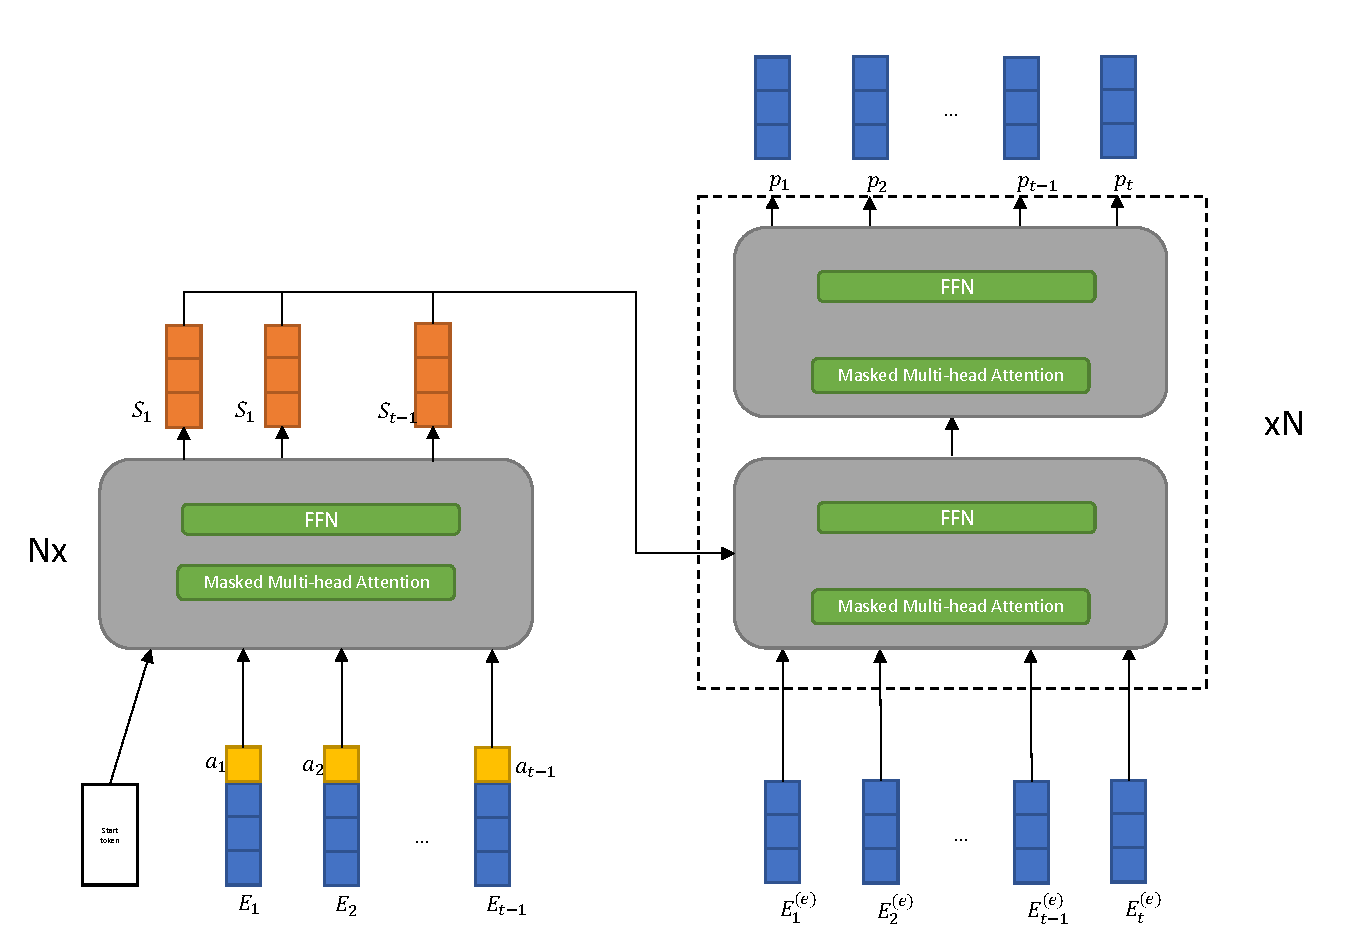
\includegraphics[width=0.9\textwidth]{ch3-trm.pdf}
	\caption{The Transformer architecture}
	\label{fig:ch3-fig5}
\end{figure}

The output of embedding layer \(E_i\) is passed into a Transformer Block, of which the first is a masked multi-head attention (MHA) module. The formula is~\ref{fml:mha}

\begin{align}\label{fml:mha}
	\begin{split}
		q_{i}   & =Q E_i                                                                \\
		k_{i}   & =K E_i                                                                \\
		v_{i}   & =V E_i                                                                \\
		A_{i j} & =\frac{q_{i} k_{j}+b(\Delta t_{i-j})}{\sqrt{d_{k}}}, \forall j \leq i \\
		h_{i}   & =\sum_{j \leq i} \operatorname{softmax}(A_{i j}) v_{j}
	\end{split}
\end{align}
Query, Key, and Value sequences are fed into the model. It separately extracts  value\(v_i\), query \(q_i\), and key \(k_i\). Then the attention from \(i\) to \(j\) can be calculated. The time difference \(b(\Delta t_{i-j})\) imports time variance into attention of \(i\) and \(j\). Then the representation of value \(i\), which is \(h_i\), can be obtained. The upper masking should be added into the MHA model to stop the effect from the current state to the future state.

The MHA output is formula~\ref{fml:mhaout}, where \(N^{(MHA)}\) is the number of head and \(W^{(Aggregate)}\) is the aggregate weight matrix.
\begin{align}
	\operatorname{MHA}(Q,K,V) = (h_1\|h_2\|\ldots \|h_t) \times W^{(Aggregate)}\label{fml:mhaout}
\end{align}

Then it is needed into the feed-forward net (FFN), which is for non-linearity import. The formula is~\ref{fml:ffn}.
\begin{align}\label{fml:ffn}
	F & = \operatorname{FFN}(\operatorname{MHA}(Q,K,V)) \\&=(F_1,F_2,\ldots,F_t)
\end{align}
The knowledge state vectors \(S_i = F_i\)

The output of FFN is actually the hidden knowledge mastery proficiency state vector. It is the output of the encoder module. In general, the Encoder formula is~\ref{fml:encoder}. The \(SkipCon(\cdot)\) is the skip connection~\cite{he2016deep} which can reduces gradient disappearance and network degradation problems, making training easier.. The \(LNorm(\cdot)\) is the Layer normalization~\cite{ba2016layer}
for normalization.
\begin{align}\label{fml:encoder}
	\begin{split}
		M^{(En)} & =SkipCon(\operatorname{MHA}(LNorm(Q,K,V))) \\
		O^{(En)} & =SkipCon(\operatorname{FFN}(LNorm(M)))
	\end{split}
\end{align}

The \(O^{(En)}\) is then as the input of Decoder's Key and Value. The Decoder apply one MHA to generate a representation of question information as formula~\ref{fml:decoder}
\begin{align}\label{fml:decoder}
	\begin{split}
		M^{(De)}_1 & =SkipCon(\operatorname{MHA}(LNorm(Q^\prime,K^\prime,V^\prime)))    \\
		M^{(De)}_2 & =SkipCon(\operatorname{MHA}(LNorm(M^{(De)}_1 ,O^{(En)},O^{(En)}))) \\
		O^{(De)}   & =SkipCon(\operatorname{FFN}(LNorm(M^{(De)}_2M)))
	\end{split}
\end{align}
The \(M^{(De)}_i\) is the ith MHA block output of decoder module. The output of decoder \(O^{(De)}\) is the prediction for exercise answering. The prediction is \(\mathbf{p}=(p_1,p_2,\ldots,p_t)\)

\section{Experiments}
%本节中,通过多个专用的知识追踪数据集来investigate提出的模型性能,与目前已经提出的Baseline模型进行性能对比。本章先对所用到的数据集进行介绍和统计,然后提出用于模型性能对比的度量标准、实验设置和运行参数环境等,最后得出结果并进行分析。
In this section, algorithms, including the performance, are investigated through multiple dedicated knowledge tracing data sets, and the performance of the proposed baseline model is compared. This chapter first introduces and counts the data sets used, then proposes metrics, experimental settings, and operating parameter environments for model performance comparison, and finally draws the results and analyzes them.


\subsection{Datasets}
After investigating the existing knowledge tracing model, the thesis selected the more popular ASSISTment data set and Statics data set related to mathematics, preprocessed the data set, cleaned the data, obtained the training set, and performed the performance with the Baseline model Compared. Dataset statistics are shown in Table~\ref{tbl:ch2-tb1}.

%(1)ASSISTment 2015 是一个用于预测学生考试表现的数据集,它由一系列包含若干知识点标签的问题以及一些学生的答题记录组成。它在2015年于线上教育平台上采集而成。经过数据过滤获得包含19917个学生,约102千个问题,100个知识点标签和约709次交互的数据集。
%(2)ASSISTment 2017 来源于2017年举办的ASSISTments Longitudinal Data Mining Competition。经过数据预处理和数据过滤,数据集包含1709个学生,4117个问题,102个知识点和约943千次交互。
%(3)Statics 2011 数据集来源于统计学课程的答题记录。
\begin{itemize}
	\item ASSISTment 2015 (ASSIST15) is a data set used to predict student test performance. It consists of a series of exercises containing several knowledge point labels and some student answer records. It was collected on an online education platform in 2015. After data filtering, a data set containing 19,917 students, about 102 thousand exercises, 100 knowledge point labels, and about 709 interactions was obtained.
	\item ASSISTment 2017 (ASSIST17) is derived from the ASSISTments Longitudinal Data Mining Competition held in 2017. After data preprocessing and data filtering, the data set contains 1709 students, 4117 exercises, 102 knowledge points, and approximately 943 thousand interactions.
	\item Statics 2011 (STATICS11) dataset is derived from the answer records of statistics courses. It contains 333 students, 1223 exercises, 156 knowledge tags, and about 189 thousand interactions.
\end{itemize}

\begin{table}[htbp!]
	\centering
	\caption{Dataset Statistics}\label{tbl:ch2-tb1}
	\begin{tabular}{ccccc}
		\toprule
		Dataset   & \#Students & \#exercises & \#Knowledge Points & \#Interactions \\
		\midrule
		ASSIST15  & 19,917     & 102,396     & 100                & 709K           \\
		ASSIST17  & 1,709      & 4,117       & 102                & 943K           \\
		STATICS11 & 333        & 1,223       & 156                & 189K           \\
		\bottomrule
	\end{tabular}
\end{table}

\subsection{Settings and Metrics}
%目前知识追踪领域的论文多以(Area Under Curve)AUC作为对比指标,AUC是一个基于ROC曲线常用的二分类评测手段,具有较好的性能对比能力。在知识追踪任务中,最终预测也是当前时刻的习题的做对与否,本质上为一个二分类问题,因此可以采取这种做法。
At present, most papers in the field of knowledge tracing use Area Under Curve (AUC) as a comparison indicator. AUC is a commonly used two-category evaluation method based on the ROC curve and has good performance comparison capabilities. In the task of knowledge tracing, the final prediction is also whether the exercises at the current moment are done correctly or not, which is essentially a binary classification problem so that this approach can be adopted.

%对于每个数据集采用70%作为训练集,剩余30%作为测试集。实验运行环境为Ubuntu20.04,TensorFlow 2.23,Python 3.8.6,实验机器为一块Tesla V100计算卡。
For each dataset, 70\% is used as the training set, and the remaining 30\% is taken as the test set. The experimental running environment is Ubuntu20.04, TensorFlow 2.23, Python 3.8.6, and the experimental machine is a Tesla V100 computing card.

\subsection{Baselines}
%1.BKT是一个知识追踪的经典模型,它基于隐马尔可夫模型(HMM),将学习者的知识状态建模为一组对应知识点掌握情况的二元变量。
%2.DKT是第一个基于深度学习的知识追踪模型,它应用将学生的做题记录输入到LSTM中,可以捕获学生做题序列上近期做题记录的影响,将学生的做题顺序考虑进模型,DKT也初步考虑了知识点间的内在相关性。
%3.GKT应用图神经网络到知识追踪任务上,利用图的特性,将知识点间的图状关联表征出来,从而更好地学习知识内在依赖关系,该模型能够学习出学生的隐藏知识状态,也具有较好的可解释性。
In this experiment, baseline performance comparisons are made by comparing some classic models with new knowledge tracing models proposed recently. The following models participate in performance comparison.
\begin{itemize}
	\item BKT~\cite{yudelson2013individualized}: BKT is a probabilistic model that predicts the probability of correctness of answers according to the basic assumption that knowledge points are independent.
	\item DKT~\cite{piech2015deep}: DKT applies the input of students' doing records into LSTM and can capture the influence of recent doing records on students' doing sequences, taking students' doing sequences into account into the model; DKT also initially considers the intrinsic correlation between knowledge points.
	\item Dynamic Key-Value Memory Networks (DKVMN)~\cite{zhang2017dynamic}: DKVMN uses key-value pairs as the memory structure, which can avoid over better prediction performance relative to BKT, and DKT is achieved by using key-value pairs as the memory structure.
	\item Graph-Based Knowledge Tracing (GKT)~\cite{nakagawa2019graph}: GKT applies graphical neural networks to knowledge tracing tasks, using the properties of graphs to characterize the graph-like associations between knowledge points for better learning of intrinsic knowledge dependencies, and the model is able to learn students' hidden knowledge states and also has better interpretability.
\end{itemize}

\subsection{Result and Analysis}
%实验结果见表,相比于其他模型,提出的模型的性能取得了最优的指标。在所有数据集上,DKT、DKVMN和GKT的标签明显优于BKT模型。在ASSIST15数据集上,提出的模型的AUC值较其他模型高出0.5\%,而GKT的性能优于DKVMN和DKT,这是由于该数据集中的知识点隐藏关联较高,因此能够更好表征知识点内在关联的模型就会明显产生更好的结果。在ASSIST17数据集上,提出的模型略优于对比的模型,而DKT、DKVMN和GKT的性能表现差异较小,这是因为知识点间的关联较小,因此考虑知识点间关联带来的性能提升较小。在STATICS11数据集上,DKVMN的性能表现超越了GKT,其原因在于对知识进行关系建模产生了过拟合现象,因此对性能表现产生了负面影响,结果显示出提出的模型抗过拟合性能较好。

The experiment's aggregated result is shown in Table~\ref{tbl:ch3-tb2}, and the proposed model achieves better performance metrics compared to other baseline models. The labels of DKT, DKVMN, and GKT are significantly better than the BKT model on all datasets. On the ASSIST15 dataset, the AUC value of the proposed model is 0.5\% higher than the other models, while GKT outperforms DKVMN and DKT due to the high hidden association of knowledge points in this dataset, so the model that can better characterize the intrinsic association of knowledge points significantly produces better results. On the ASSIST17 dataset, the proposed model slightly outperforms the compared models. Simultaneously, the performance difference between DKT, DKVMN, and GKT is more minor due to the minor association between knowledge points, and thus the performance improvement from considering the association between knowledge points is more diminutive. On the STATICS11 dataset, the performance of DKVMN outperforms GKT due to the overfitting phenomenon arising from modeling the relationship to knowledge, thus negatively affecting the performance, and the results show that the proposed model has better performance against overfitting.

\begin{table}[htbp!]
	\centering
	\caption{AUC results (\%) over three datasets}\label{tbl:ch3-tb2}
	\begin{tabular}{cccc}
		\toprule
		Model    & ASSIST15                    & ASSIST17                   & STATICS11                  \\
		\midrule
		BKT      & \(62.01\pm 0.03 \)          & \(65.30\pm 0.01\)          & \(64.21\pm 0.01\)          \\
		DKT      & \(70.83\pm 0.03 \)          & \(72.66\pm 0.01\)          & \(72.46\pm 0.06\)          \\
		DKVMN    & \(71.06\pm 0.03 \)          & \(72.78\pm 0.02\)          & \(72.67\pm 0.03\)          \\
		GKT      & \(72.12\pm 0.02 \)          & \(72.85\pm 0.01\)          & \(72.57\pm 0.01\)          \\
		\midrule
		Proposed & \(\mathbf{72.62\pm 0.02} \) & \(\mathbf{72.89\pm 0.02}\) & \(\mathbf{72.73\pm 0.02}\) \\
		\bottomrule
	\end{tabular}
\end{table}
\section{Summary}
%
In this section, a knowledge tracing model based on graph self-attentive network hungry embedding with Transformer is proposed, which learns the relationship between exercises and knowledge points through GAT, which can effectively characterize the complex dependencies between knowledge points and can discover the hidden knowledge points in the exercises. In the encoding part, the embedding vectors learned by GAT are encoded by a Transformer model for knowledge state, and a knowledge state sequence is an output, which can be used in the subsequent exercise recommendation process. At the same time, the knowledge state sequence and the exercises are used as the input of the subsequent Decoder to output a simulation of the correct or incorrect answers to the exercises.

The innovation points of this section are as follows.
\begin{enumerate}
	\item Based on the graph self-attentive network, a relational graph network with separation of exercises and knowledge points are designed, and the knowledge state embeddings learned in this way can better characterize the intrinsic dependencies of knowledge points.
	\item Through the encoder based on Transformer block, the intrinsic knowledge state vector of students is output, and this state vector can be used for subsequent learning resource recommendation.
	\item With the Transformer block, bidirectional sequence information can be learned better to model students' knowledge states' change.
\end{enumerate}

The model is experimentally verified to achieve good prediction performance for both datasets with closely linked knowledge points and those with sparse knowledge point relationships, and overfitting can also be prevented by proper tuning of parameters.